\documentclass{article}
\usepackage{anuragLatexArticleStyle}
\usepackage[utf8]{inputenc}

\title{Kilobotics}
\author{Anurag (183230006)\\ Eswara Srisai \\ Sudhakar \\ Kishan}
\date{\today}

\begin{document}

\maketitle

\section{Introduction}
Kilobots are small robots with following specifications
\begin{itemize}
    \item One IR transmitter-receiver pair
    \item One ambient light sensor
    \item Two vibrators to move robot using stick and slide mechanism
    \item One onboard battery
    \item One RGB LED
\end{itemize}
\begin{figure}[H]
    \centering
    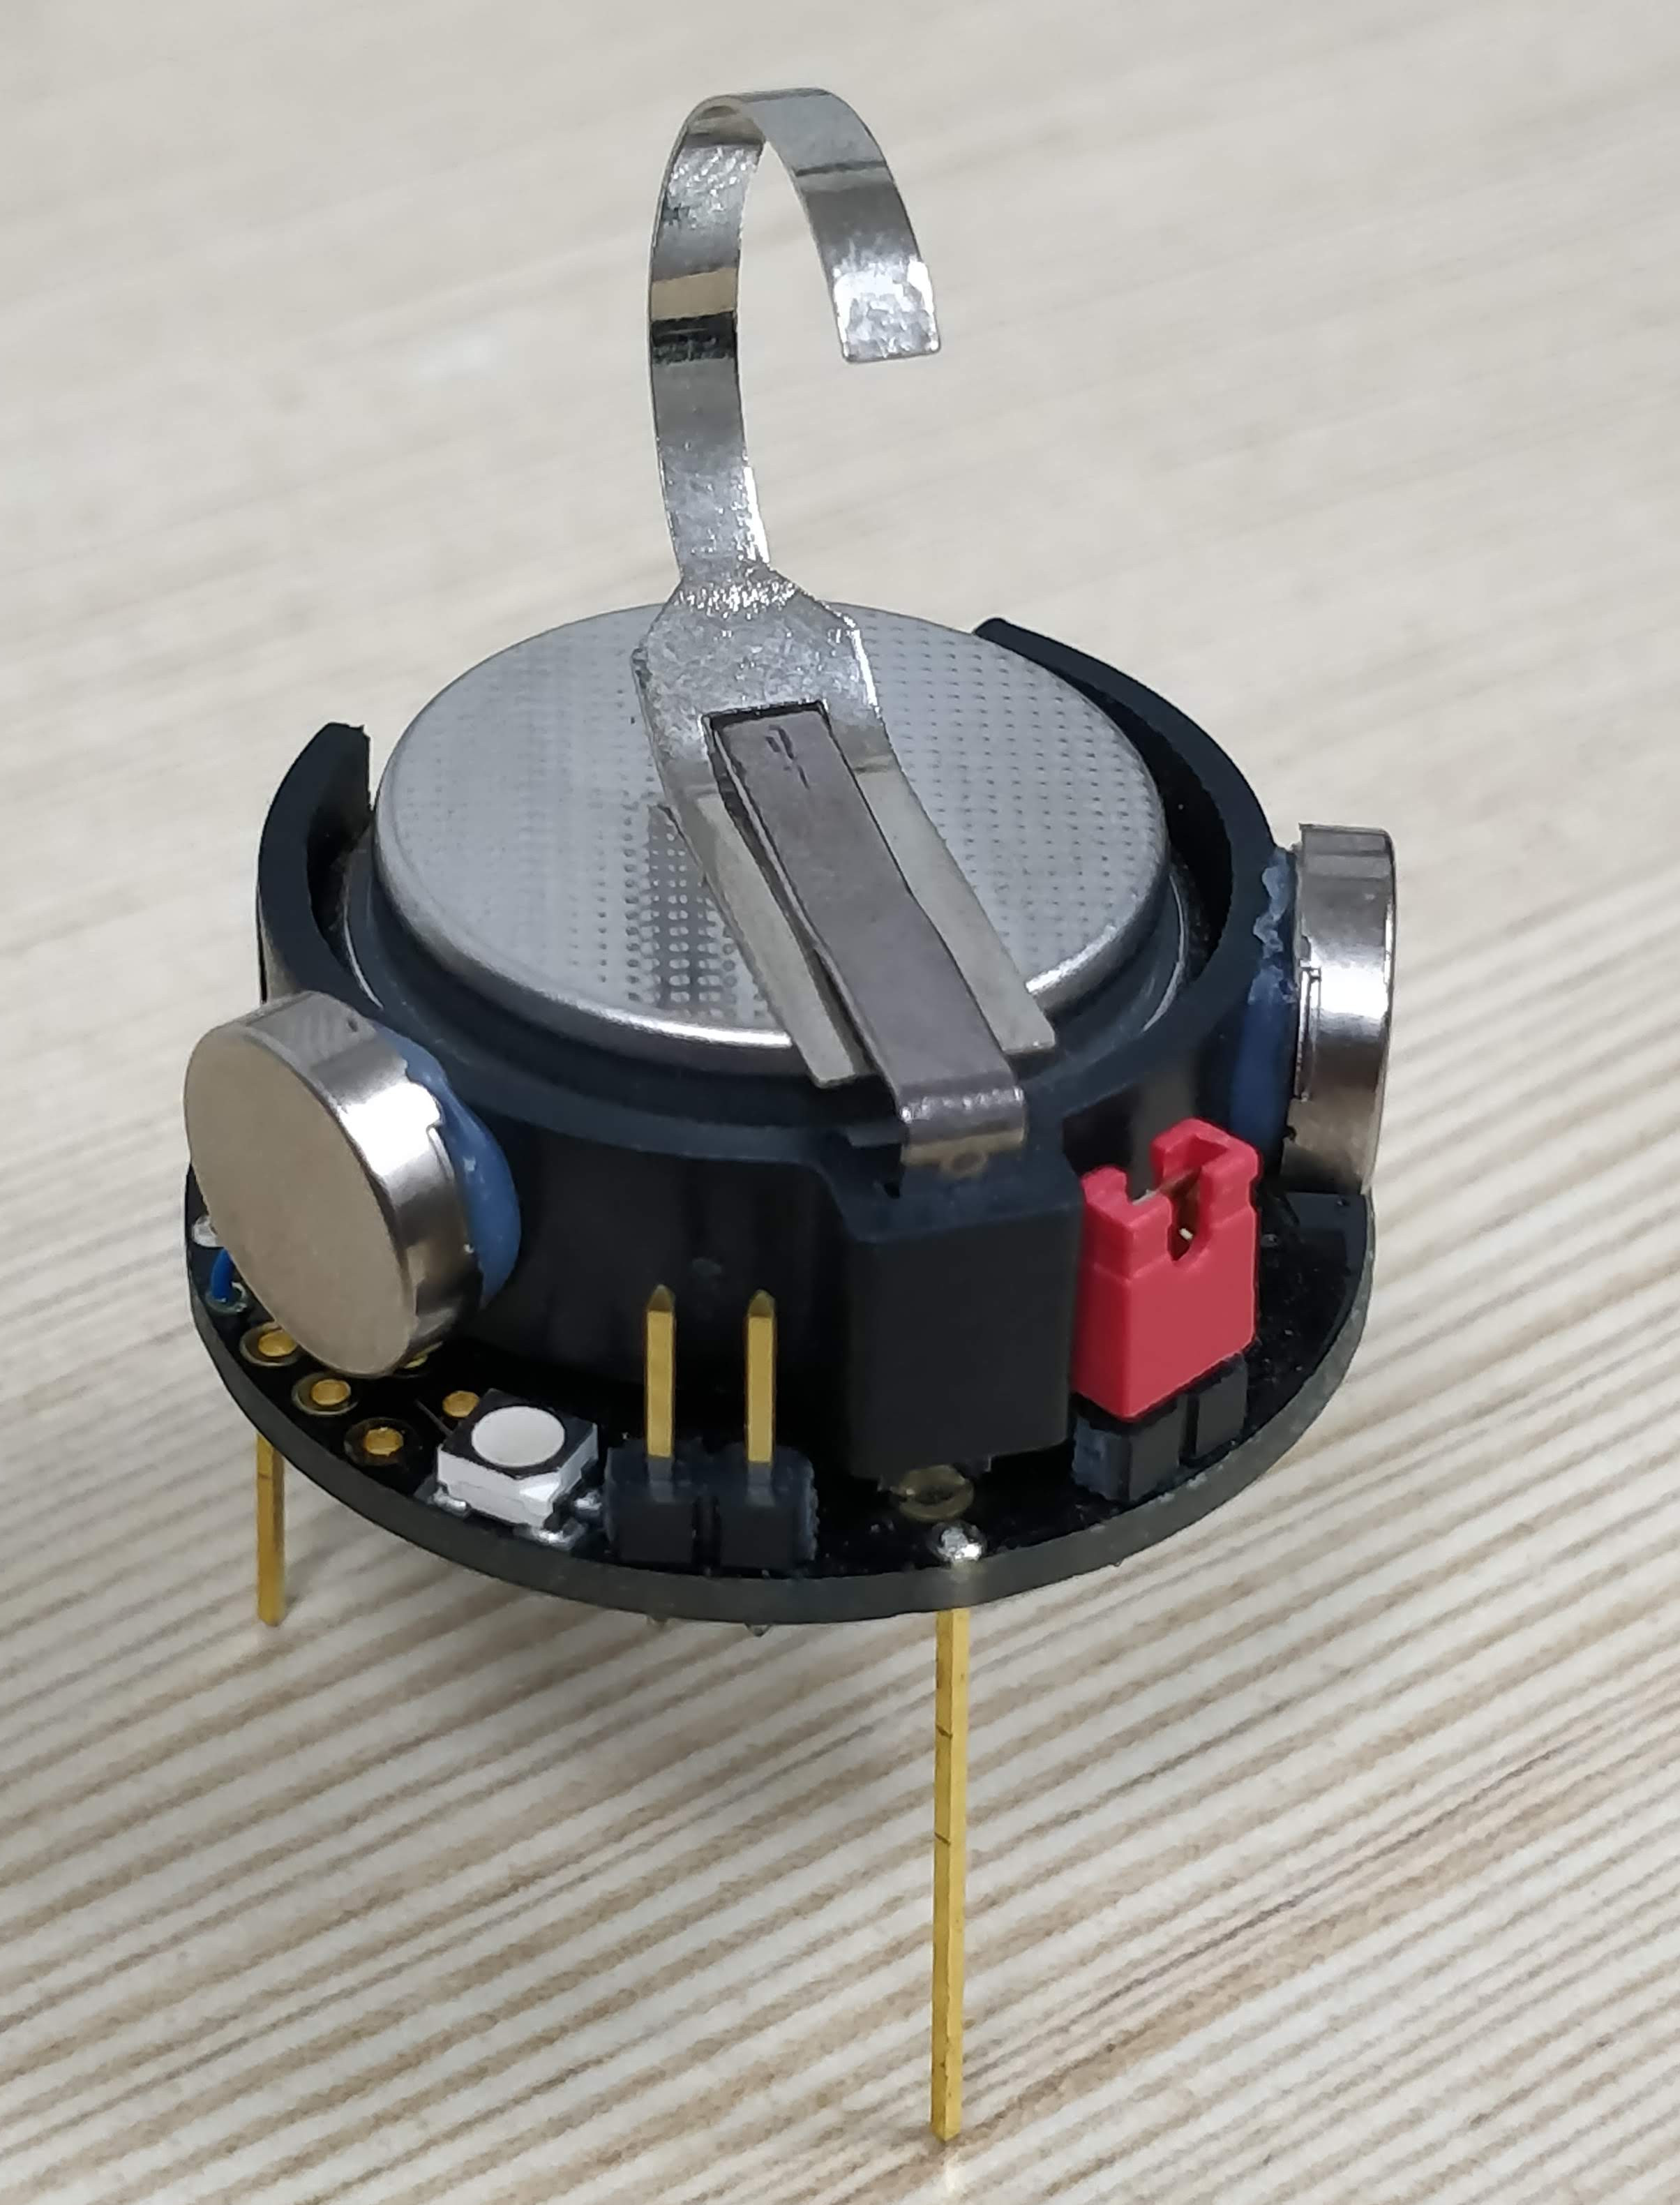
\includegraphics[scale=0.04]{images/kilobots}
    \caption{Kilobots}
\end{figure}

\section{Communication}

\section{Planet orbiting a star}

\section{Robot moving towards the light source}
The problem statement is similar to a line follower with just one onboard sensor. The algorithm for single sensor line follower goes as follows:
\begin{enumerate}
    \item Check sensor position.
    \item If sensor is on line, go to step 3 else step 4.
    \item Move right. Go to step 5.
    \item Move left.
    \item Go to step .
\end{enumerate}
On similar lines, following a light source algorithm goes as follows:
\begin{enumerate}
    \item Check ambient light sensor value.
    \item If ambient light is less than THRESHOLD\_LOW, go to step 3 else if ambient light is greater than THRESHOLD\_HI go to step 4, otherwise go to step 5.
    \item Move left. Go to step 6.
    \item Move right. Go to step 6.
    \item Continue previous motion.
    \item Go to step 1.
\end{enumerate}
\subsection{Demonstration}
\begin{figure}
    \centering
    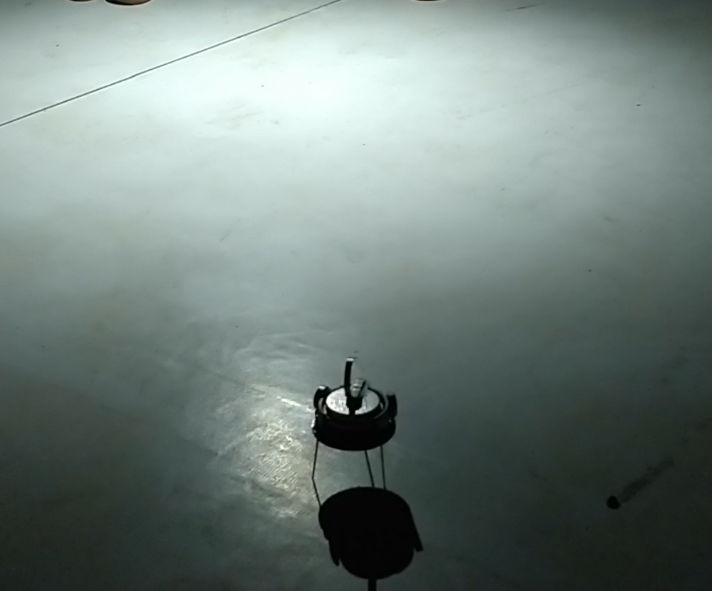
\includegraphics[scale=0.4]{images/move_towards_light}
    \caption{Move towards the light source}
\end{figure}
\section{Syncing phase of blinking LEDs}

\end{document}

